\chapter{Forschungsbedarf und -ansatz}

Ziel dieser Arbeit ist die Erarbeitung eines Konzepts für die Nutzung von Rechenressourcen in autonomen Fahrzeugen. Ein solches Konzept soll möglichst allgemein verwendbar sein, mit möglichst geringer Abhängigkeit zur eingesetzter Hardware und Betriebssystem. Zudem soll die Kommunikationsschnittstelle flexibel gestaltet werden, um die Integration in bestehenden Kommunikationsprotokolle zu vereinfachen. Hierfür wird eine entsprechend geeignete Struktur vorgesehen mit definierten Schnittstellen. In dieser Arbeit werden die Anforderungen ermittelt, die für die Nutzung von Rechenressourcen in Fahrzeugen relevant sind. Anhand der ermittelten Anforderungen werden die vorhandenen technische Lösungen bewertet und ein geeigneter Ansatz und Architektur erarbeitet.

\section{Forschungsbedarf}

Im folgenden Abschnitt wird der Forschungsbedarf anhand der Stand der Technik aus Kapitel 2 vorgestellt. Hierfür werden die Methoden für Applikationsmanagement betrachtet, die in IT Infrastrukturen verwendet werden und deren Eignung für den Einsatz in Fahrzeugen. 

\subsection{Virtualisierung}
Im \autoref{Applikationsmanagement} wurden die gängigen Virtualisierungsmethoden vorgestellt, die vorwiegend in IT Infrastruktur zur Verwendung kommen. Diese bilden die Grundlage für Applikationsmanagement in IT Systemen. Diese Methoden können grundsätzlich auch für Fahrzeugsteuergeräte verwendet werden, allerdings unterscheiden sich die Steuergeräte in Hardwarekomponenten und Betriebssystem, so dass die vorhandene Lösungen aus dem IT Bereich nicht unmittelbar verwendet werden können. Um eine möglichst hohe Kompatibilität für verschiedene Architekturen zu gewährleisten, müssen die Virtualisierungsmethoden für verschiedene Architekturen verfügbar oder portierbar sein. Vorteilhaft sind hierbei Lösungen, die mit offenem Quellcode, da hier die Portierung je nach Lizenzbedingungen auch unabhängig vom Entwickler vorgenommen werden kann. Im Allgemeinen muss eine Virtualisierungstechnologie, die auf verschiedenen Plattformen zum Einsatz kommen soll, eine einfache Portierbarkeit gewährleisten. Aktuelle IT-Lösungen gewährleisten die Kompatibilität mit gängigen Hardware-Plattformen und Betriebssystemen. Die gängigste Hardwarearchitektur in IT Infrastrukturen ist die x86 Architektur, diese ist allerdings nicht gut geeignet für sicherheitskritische Echtzeitapplikationen, da das System Management Mode kein deterministisches Verhalten für Betriebssystem und Applikationen zulässt. Autonome Fahrzeugsteuergeräte verwenden Architekturen, wo die Echtzeitfähigkeit garantiert werden kann. Die Portierbarkeit auf diese anderen Hardwarearchitekturen von Fahrzeugsteuergeräten stand bei der Entwicklung der Virtualisierungslösungen nicht im Vordergrund. Virtuelle Maschinen erfordern die hardwareseitige Unterstützung von Virtualisierungsmethoden, so dass diese Art von Virtualisierung schwieriger zu portieren ist. Containerisierung nutzt bestimmte Linux Kernelfeatures, so dass hier eine Einschränkung seitens Betriebssystem auf dem Zielgerät stattfindet. 

Software und Hardware im Automobil müssen Sicherheitsstandards erfüllen. Dazu wurde die Norm ISO 26262 entwickelt. \cite{Birch2013} Wenn also eine Virtualisierungsmethode im Steuergerät des Fahrzeugs eingesetzt wird, muss sie auch nach der Norm ISO 26262 geprüft werden. In diesem Prozess müssen mögliche Gefahren, die sich aus einer Fehlfunktion des Systems ergeben, identifiziert und ihr Schweregrad bestimmt werden. Je umfangreicher der Funktionsumfang der Software ist, desto aufwendiger ist diese Zertifizierung, da damit auch die Anzahl der möglichen Fehlfunktionen steigt. Virtualisierungslösungen aus der IT sind auf universelle Einsetzbarkeit optimiert und bieten dafür eine Vielzahl von Funktionalitäten, von denen viele je nach Anwendungsfall nicht relevant sind. Der hohe Funktionsumfang erhöht jedoch den Aufwand für die Zertifizierung nach ISO 26262.

\subsection{Orchestrierung}
Für die Orchestrierung von virtuellen Umgebungen existiert eine Vielzahl von Anwendungen die im \autoref{Orchestrierung Stand der Technik} vorgestellt wurden. Aus \autoref{Verteiltes Rechnen in Fahrzeugen} geht hervor, dass die Orchestrierung von Applikationen in Fahrzeugen ein aktuelles Forschungsfeld ist, wo stand jetzt (2024) keine fertige kommerzielle Lösungen existieren. Aus funktionaler Sicht sind die Orchestrierungsapplikationen aus der IT auch für die Orchestrierung von Fahrzeugapplikationen geeignet. Ein wesentlicher Unterschied zwischen der Orchestrierung verteilter IT-Systeme und Fahrzeugen besteht in der Dynamik, mit der sich die Eigenschaften der Systeme ändern. Verteilte Systeme im IT Bereich bestehen üblicherweise aus einzelnen Server oder Rechencluster, die verwaltet werden. Die Verfügbarkeit der Systeme ist hoch, sie gehen nur im Fehlerfall oder bei geplanten Wartungen offline. Die verfügbaren Rechenressourcen sind ebenfalls einfach kalkulierbar, da die Systeme in der Regel nur die Applikationen ausführen, die sie vom Orchestrierer erhalten. Die Orchestrierung der ungenutzten Rechenressourcen von Fahrzeugen ist im Vergleich mit einem signifikanten Mehraufwand verbunden. Die Rechenressourcen von Fahrzeugsteuergeräten werden primär für fahrzeuginterne Funktionen genutzt. Die Menge an verfügbaren Ressourcen für externe Applikationen ist hierdurch stark vom Fahrzeugzustand abhängig und kann sich entsprechend dynamisch ändern. Zusätzlich unterliegt auch die Qualität Netzwerkanbindung von Fahrzeugen erhebliche Schwankungen. Dies erfordert eine erweiterte Parameterbetrachtung und Abschätzung zukünftiger Zustände im Vergleich zu den derzeit üblichen Maßnahmen, die bei der Orchestrierung verteilter Systeme eingesetzt werden.
 
\subsection{Verteiltes Rechnen in Fahrzeugen}

Die Bereitstellung der Ressourcen von Fahrzeugen für externe Anwendungen stellt ein aktuelles Forschungsfeld dar. Im \autoref{Verteiltes Rechnen in Fahrzeugen} wurde ein Überblick über die Forschungsthemen in diesem Gebiet aufgezeigt. In diesem Kontext wurde bereits aufgezeigt, dass es noch keine marktreife Lösungen existieren. Derzeit sind die meisten auf dem Markt erhältlichen Fahrzeuge noch nicht in der Lage, die erforderlichen technischen Voraussetzungen für eine sinnvolle externe Ressourcennutzung zu erfüllen. Die technische Entwicklung geht jedoch eindeutig in Richtung zunehmender Automatisierung und damit verbundener zentralisierter \glsxtrshort{E/E} Architekturen mit entsprechend leistungsfähigeren Steuergeräten. Es ist daher zu erwarten, dass dieses Thema in der Zukunft erheblich an Relevanz gewinnen wird. Die meisten aktuellen Forschungsansätze sind theoretischer oder simulativer Natur, funktionale Umsetzungen gibt es kaum. 

\subsection{Ableitung des Forschungsbedarfs}

Zusammenfassend lässt sich ableiten, dass die Entwicklung einer Plattform, die spezifisch auf die Orchestrierung von externen Anwendungen auf Fahrzeugen zugeschnitten ist, als sinnvoller Schritt erachtet werden kann. Aktuelle Forschungsansätze diskutieren mögliche Einsatzgebiete und die theoretische Machbarkeit eines solchen Systems, ausgereifte Umsetzungen existieren aktuell nicht. Bei der konkreten Umsetzung können auch Aspekte wie Portierbarkeit auf andere Architekturen und Kompatibilität mit fahrzeugspezifischen Betriebssystemen berücksichtigt werden. Darüber hinaus können Mindestfunktionalitäten identifiziert werden, die helfen, ein solches System nicht mit unnötigen Funktionen zu überfrachten und damit die Systemanforderungen und die Sicherheit zu beeinträchtigen. Als Grundlage kann auf bestehende Orchestrierungs- und Managementmethoden aus der IT sowie auf bereits erarbeitete Ansätze aus dem Stand der Technik für verteiltes Rechnen im Fahrzeug zurückgegriffen werden.

\section{Anforderungsanalyse}
\label{Anforderungsanalyse}

Die Anforderungsanalyse ist eine verbreitete Methode für die Entwicklung von technischen Systemen. Produktentwicklungen werden heutzutage nicht mehr von einem Designingenieur geleitet, sondern von einem Team von Spezialisten. Um sicherzustellen, dass alle Komponenten, die die Spezialisten entwerfen, zusammenspielen und den Kundenwünschen entsprechen, werden Anforderungen definiert. Diese Anforderungen werden in funktionale und nicht-funktionale Anforderungen unterteilt. \cite{Grady2010}

\subsection{Funktionale Anforderungen}

Funktionale Anforderungen sind Anforderungen, die für die Zweckbestimmung des Produkts relevant sind. Bei einem Softwareprodukt werden sowohl die Funktionen die die gesamte Anwendung implementieren soll als auch die Funktionen der einzelnen Komponenten darin definiert. 

\begin{itemize}
    \item 1: Die Softwareplattform soll es ermöglichen, externe Applikationen in Fahrzeugsteuergeräten zu platzieren, um deren Rechenleistung zu nutzen.
    \item 2: Die im Netz verfügbaren Fahrzeuge müssen automatisch als mögliche Auslagerungsorte erkannt werden.
    \item 3: Fahrzeuge müssen deren Verfügbarkeit sowie deren freie Ressourcen mitteilen, um eine sinnvolle Auslagerung der Applikationen zu ermöglichen
    \item 4: Auf dem Fahrzeugsteuergerät muss eine eigene Laufzeitumgebung für die externe Applikationen errichtet werden
    \item 5: Die im Fahrzeug ausgelagerte externe Applikationen müssen eine Kommunikationsschnittstelle erhalten
\end{itemize}

An dieser Stelle wird auf eine genaue Vorgabe für die verwendeten Methoden oder Architektur verzichtet. Die gewählte Lösung soll lediglich den gestellten Anforderungen gerecht werden. 

\subsection{Nicht-funktionale Anforderungen}

Nicht-funktionale Anforderungen beschreiben in erster Linie Anforderungen, die sich auf die Qualität auswirken. Produktentwicklungen, die die nicht-funktionalen Anforderungen nicht erfüllen, sind zwar funktional, erfüllen aber nicht die vom Kunden gewünschte Nutzererfahrung. Bei Softwareprodukten fallen beispielweise Leistung, Sicherheit oder Wartbarkeit in diese Gruppe. 

\begin{itemize}
    \item 1: Applikationen sollen von der Funktionssoftware im Fahrzeug isoliert sein um unberechtigte Zugriffe auf Fahrzeugdaten zu verhindern
    \item 2: Es soll eine Authentifizierung bei der Netzwerkkommunikation vorgesehen werden um unberechtigte Zugriffe zu verhindern
    \item 3: Die Kommunikationsschnittstellen sollen modular und austauschbar ausgelegt werden um die Kompatibilität zu erhöhen
    \item 4: Die Virtualisierungsapplikation für die Fahrzeugsteuergeräte soll möglichst einfach auf verschiedene Hardwarearchitekturen portierbar sein
    \item 5: Funktionsumfang der Virtualisierungsapplikation soll für eine einfachere Sicherheitsbetrachtung möglichst auf die notwendige Funktionen zugeschnitten sein
\end{itemize}

Die Sicherheitsbetrachtung steht nicht im Fokus dieser Arbeit, da dies ein komplexes Feld ist wo die Entwicklung bereits sehr fortgeschritten ist, da es für sehr viele Applikationen Relevanz besitzt. 

\section{Methodik}

In der Softwareentwicklung gibt es eine Vielzahl von Mustern, die für die Produktentwicklung genutzt werden können. \cite{Bass2012} In dieser Arbeit wird die Vorgehensweise an das V-Modell angelehnt. Eine Schematische Darstellung kann in der Abbildung \ref{v-model} betrachtet werden. Auf der Grundlage der in der Anforderungsanalyse ermittelten Anforderungen werden die Spezifikationen für die Software erstellt. Daraus werden in der nächsten Phase die Softwarearchitektur und das Design abgeleitet. Anschließend werden die einzelnen Komponenten spezifiziert. Nach der Implementierung der Komponenten erfolgt die Validierung der Komponenten gegen die Komponentenspezifikationen. Im nächsten Schritt werden die Komponenten in die Gesamtarchitektur integriert und gegen die Architekturspezifikationen validiert. Die integrierten Komponenten ergeben das System. Hier erfolgt die Validierung gegen die Systemspezifikationen. Abschließend wird das fertige Produkt durch Abnahmetests gegen die Systemanforderungen validiert. Falls Abweichungen zu den Spezifikationen festgestellt werden, wird das V-Modell iterativ nochmal durchgelaufen. 

\begin{figure}[htbp]
	\centering
	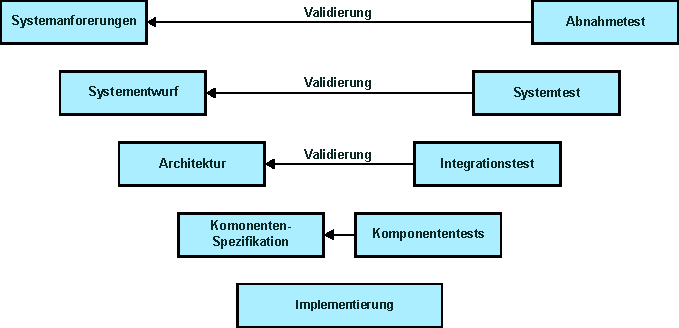
\includegraphics[width=\textwidth]{./content/graphics/V-model.pdf}
	\caption{Das V-Modell in der Softwareentwicklung}
	\label{v-model}
\end{figure}

[Einordnung des V-Modells in die Struktur der Arbeit]

\section{Forschungsansatz}
Ausgehend von den identifizierten Defiziten bestehender Systeme wird ein Konzept und eine prototypische Implementierung einer Plattform vorgenommen, die es ermöglicht, externe Applikationen auf Fahrzeugsteuergeräten zu verwalten. Hierzu muss zunächst ein Konzept gewählt werden, das die gestellten Anforderungen erfüllt. Zunächst muss die verwendete Virtualisierungstechnologie festgelegt werden. Im \autoref{Applikationsmanagement} wurden die zwei Virtualisierungsmethoden aus der Informationstechnik vorgestellt. Die Hardwarevirtualisierung mit virtuellen Maschinen bietet mehr Flexibilität und eine größere Isolation vom verwendeten System, aber diese Virtualisierungsmethoden müssen an die jeweilige Hardwarearchitektur angepasst werden und verursachen mehr zusätzlichen Rechenaufwand als die Softwarevirtualisierung. Software-Virtualisierung mittels Containern ist mit den meisten Linux-Distributionen nativ realisierbar. Leistungsfähige Fahrzeugsteuergeräte verwenden in der Regel eine angepasste Linux Distribution als Betriebssystem, so dass die Software Virtualisierung in den meisten Fällen ohne zusätzliche Anpassungen im Betriebssystem einsetzbar ist. Damit ist diese Methode deutlich einfacher auf verschiedene Steuergeräte portierbar. Aus diesem Grund wird die höchste Kompatibilität dann erreicht, wenn diese Virtualisierungsmethode eingesetzt wird.